\documentclass[]{llncs} % "you can ignore this hint if your document works"
\usepackage{makeidx}
\usepackage{graphicx}
\usepackage{makecell}
\usepackage{float}
\begin{document}
\addtocmark{Southern Methodist University}

\title{Machine Learning Predicts Aperiodic Laboratory Earthquakes}
\author{Olha Tanyuk, Daniel Davieau, Charles South \and Daniel W. Engels}
\institute{Southern Methodist University, Dallas TX 75205, USA \newline otanyuk@mail.smu.edu, danieldavieau@mail.smu.edu, csouth@mail.smu.edu, dwe@lyle.smu.edu }


\maketitle
\begin{abstract}
In this paper we use .3 second time intervals to identify a pattern of aperiodic seismic signals that precede earthquakes at any time in a laboratory earthquake’s cycle. We apply machine learning to a data set collected from a laboratory experiment in which several stick-slip displacements (earthquakes) occur. This type of experiment  has been studied in depth as a simulation of seismologic faults for decades. The data exhibits similar behavior to natural earthquakes, so the same approach may work in predicting the timing of natural earthquakes. Here we show that by applying a random forest regression algorithm to the acoustic signal emitted by a laboratory fault, we can predict the time remaining before a failure occurs with 1.61 seconds mean absolute error at any moment of earthquake’s cycle. These predictions are based solely on acoustical signal's statistical features derived from local, moving 0.3 second time windows and do not make use of its history. Essential improvements in providing new understanding of fault physics may be brought by applying this technique to acoustic seismic data.\par
\end{abstract}

\section{Introduction}
Earthquakes cause mass destruction and loss of life. A traditional method to predict earthquakes is to look to past recurrence intervals. Because the recurrences are not constant, predictions can only be made within broad time windows. One such model predicted that a strong earthquake would occur between 1985 and 1993 in the Parkfield California area but no significant event actually occurred until 2004 \cite{Jackson}. \par

Advances in instrumentation quality and density have fostered hope that progress can be made in forecasting. These advances have led to discoveries of previously unidentified slip processes such as slow slips. Slow Slip Earthquakes (SSE) are fault behaviors that occur slowly enough to make them undetectable without instrumentation. They do not cause immediate widespread destruction like regular earthquakes do. They occur near the boundaries of large earthquake rupture zones \cite{Slip}. There is evidence to suggest that there is a relationship between slow slip earthquakes and more noticeable regular earthquakes \cite{SlowSlip}. \par

Researchers imitate natural slow slip earthquakes in the laboratory by placing rocky material between steel blocks and applying shear stress to induce slipping. Recent improvements in the instruments \cite{kaggle} used to measure signals have enabled the collection of larger volume data that akin to natural earthquakes. However, processing the data and detecting patterns in it has become more difficult to work with. The ways to detect patterns of aperiodic seismic signals that precede earthquakes are presented in this paper. We use acoustic data provided by the Los Alamos National Laboratory (LANL) as part of a 2019 Kaggle competition \cite{kaggle}, which also represents laboratory slow-slip earthquakes. The data is very aperiodic and more akin to natural earthquakes than the data LANL studied earlier in 2017 \cite{kaggle}. We predict laboratory earthquakes given aperiodic slow-slip failures. We demonstrate that random forest regression can be used to detect patterns in the data that close to natural and predict laboratory earthquakes with 1.61 seconds mean absolute error. Given seismic signal data with considerably more aperiodic slow-slip laboratory earthquake failures, we predict time remaining before failure at any time in the slip cycle based solely on acoustical signal's statistical features derived from the small, local, moving time windows and do not make use of its history.\par

The results of this experiment are potentially applicable to the field of real world earthquakes \cite{Bertrand}. Essential improvements in providing new understanding of fault physics may be brought by applying this technique to acoustic seismic data. Other potential applications include avalanche prediction, landslides and failure of machine parts \cite{Bertrand}. \par

\section{Earthquakes}
An earthquake is the shaking of the surface of the Earth, resulting from the sudden release of energy in the Earth’s lithosphere that creates seismic waves. It happens when two blocks of the earth suddenly slip past one another. The surface where they slip is called the fault or fault plane \cite{Wald}. The location below the earth’s surface where the earthquake starts is called the hypocenter, and the location directly above it on the surface of the earth is called the epicenter \cite{Wald}. \par
Smaller earthquakes that happen in the same place as the larger earthquake that follows are called foreshocks. Scientists can’t tell that an earthquake is a foreshock until the larger earthquake happens \cite{Wald}. The largest, main earthquake is called the mainshock \cite{Wald}. Mainshocks always have aftershocks that follow, smaller earthquakes that occur afterwards in the same place as the mainshock \cite{Wald}. Depending on the size of the mainshock, aftershocks can continue for weeks, months, and even years after the mainshock \cite{Wald}.\par
The earth has four major layers: the inner core, outer core, mantle and crust \cite{Wald}. The crust and the top of the mantle make up a thin skin on the surface of our planet; this skin is not all in one piece – it is made up of many pieces like a puzzle covering the surface of the earth \cite{Wald}. These puzzle pieces are called tectonic plates, and the edges of the plates are called the plate boundaries. Tectonic plates keep slowly moving around, sliding past one another and bumping into each other. The plate boundaries are made up of many faults, and most of the earthquakes around the world occur on these faults \cite{Wald}. Since the edges of the plates are rough, they get stuck while the rest of the plate keeps moving \cite{Wald}. Finally, when the plate has moved far enough, the edges unstick on one of the faults and there is an earthquake \cite{Wald}. \par
While the edges of faults are stuck together, and the rest of the block is moving, the energy that would normally cause the blocks to slide past one another is being stored up \cite{Wald}. When the force of the moving blocks finally overcomes the friction of the jagged edges of the fault and it unsticks, all that stored up energy is released \cite{Wald}. The energy radiates outward from the fault in all directions in the form of seismic waves, those waves shake the earth as they move through it, and when the waves reach the earth’s surface, they shake the ground and anything on it \cite{Wald}. \par
The size of an earthquake depends on the size of the fault and the amount of slip on the fault, but that’s not something scientists can simply measure with a measuring tape since faults are many kilometers deep beneath the earth’s surface \cite{Wald}. The strength of shaking from an earthquake diminishes with increasing distance from the earthquake's source, so the strength of shaking at the surface from an earthquake that occurs at 500km deep is considerably less than if the same earthquake had occurred at 20 km depth \cite{Wald}. The size of the earthquake is called its magnitude. The Richter Scale (ML) is what most people have heard about, but in practice it is not commonly used anymore, except for small earthquakes recorded locally, for which ML and short-period surface wave magnitude (Mblg) are the only magnitudes that can be measured \cite{Hayes}. For all other earthquakes, the moment magnitude (Mw) scale is a more accurate measure of the earthquake size \cite{Hayes}. Moment Magnitude (MW) is based on physical properties of the earthquake derived from an analysis of all the waveforms recorded from the shaking \cite{Hayes}. First the seismic moment is computed, and then it is converted to a magnitude designed to be roughly equal to the Richter Scale in the magnitude range where they overlap \cite{Hayes}. Another way to measure the size of an earthquake is to compute how much energy it released \cite{Hayes}. The amount of energy radiated by an earthquake is a measure of the potential for damage to man-made structures \cite{Hayes}. The energy can be converted into yet another magnitude type called the Energy Magnitude (Me) \cite{Hayes}. \par
Slow Slip Earthquakes (SSE) are fault behaviors that occur slowly enough to make them undetectable without instrumentation. They do not cause immediate widespread destruction like regular earthquakes do. They occur near the boundaries of large earthquake rupture zones \cite{Slip}. Most SSE has been observed near the downdip limit of the seismogenic zone at depths of 25–45 km, but in well-instrumented areas it has also been detected at shallow depths
(less than 10 km), updip of large earthquake ruptures \cite{Slip}. SSE at tectonic boundaries probably occur at the plate interface, and therefore should be controlled by the frictional properties and conditions that characterize fault zones \cite{Slip}. For deep slow slip events, laboratory testing of natural material under in situ conditions is not feasible at present \cite{Slip}.  

\section{Los Alamos National Laboratory's Findings}
In 2017 Los Alamos National Laboratory (LANL) researchers discovered a way to successfully predict Slow Slip Earthquakes (SSE) in a laboratory experiment that simulates natural conditions. The team trained a computer to pinpoint and analyze quasi‐periodic seismic and acoustic signals emitted during the movements along the fault. They processed massive amounts of data and identified a particular sound pattern previously thought to be noise that precedes an earthquake. The team was able to characterize the time remaining before a laboratory earthquake at all times using a time window of 1.8 sec of the data to make each prediction with 89\% coefficient of determination \cite{LANLNews}. This result was achieved using a Random Forest Regression machine learning technique and quasi‐periodic data. \par
In the lab, the team imitated a real earthquake using steel blocks interacting with rocky material to cause slipping that emitted seismic sounds. An accelerometer recorded the acoustic emission emanating from the sheared layers \cite{LANLNews}. For the first time, researchers discovered a pattern that accurately predicted when a laboratory earthquake would occur. The LANL team acknowledges that the characteristics of the lab experiment such as shear stress differ from natural earthquakes but the application of the analysis to the real world to validate their results is ongoing. This method can also be applied outside of seismology to support material failure research in other fields such as aerospace and energy \cite{LANLNews}. The lab results reveal that the fault does not fail randomly but in a predictable manner. The observations also demonstrate that the fault’s critical stress state which indicates when it might slip can be determined using exclusively an equation of state \cite{LANLNews}. So far seismologists and earth scientists have mostly relied on catalogs of historical data to try to characterize the state of faults. These catalogs contain a minute fraction of seismic data with portions discarded during analysis as useless noise. The authors discovered that hidden in the noise-like data are signals that inform them of the state of the fault much more precisely than catalogs \cite{LANLNews}. \par

\section{Random Forest Overview}
Random Forest (RF) is an ensemble machine learning technique capable of performing both regression and classification tasks using multiple decision trees and a statistical technique called bagging \cite{RandomForest}. Decision trees are predictive models that use a set of binary rules to calculate a target value \cite{RandomForest}. Each individual tree is a fairly simple model that has branches, nodes and leaves  \cite{RandomForest}. A sub section of entire tree is called branch or sub-tree. Root Node represents entire population or sample and this further gets divided into two or more homogeneous sets. Nodes that do not split are called Leaves. A decision tree is arriving at an estimate by asking a series of questions to the data, each question narrowing our possible values until the model get confident enough to make a single prediction \cite{RandomForest}. The order of the questions (the questions asked are all in a True/False form) as well as their content are being determined by the model \cite{RandomForest}.
A RF, instead of just averaging the prediction of trees, uses two key concepts that give it the name random: \par
1. Random sampling of training observations when building trees.\par
2. Random subsets of features for splitting nodes.\par
In other words, Random forest builds multiple decision trees and merge their predictions together to get a more accurate and stable prediction rather than relying on individual decision trees \cite{RandomForest}.\par
Each tree in a random forest learns from a random sample of the training observations \cite{RandomForest}. The samples are drawn with replacement, known as bootstrapping, which means that some samples will be used multiple times in a single tree \cite{RandomForest}. The idea is that by training each tree on different samples, although each tree might have high variance with respect to a particular set of the training data, overall, the entire forest will have lower variance but not at the cost of increasing the bias \cite{RandomForest}. \par
The fundamental idea behind a random forest is to combine the predictions made by many decision trees into a single model \cite{RandomForest}. Individually, predictions made by decision trees may not be accurate but combined together, the predictions will be closer to the true value on average \cite{RandomForest}.\par
Let's understand Random Forest step by step in below example:
Step 1: Samples are taken repeatedly from the training data so that each data point is having an equal probability of getting selected, and all the samples have the same size as the original training set \cite{RandomForest}.\par
Let's say we have the following data:\par
x= 0.1,0.5,0.4,0.8,0.6, y=0.1,0.2,0.15,0.11,0.13 where x is an independent variable with 5 data points and y is dependent variable \cite{RandomForest}.\par
Now Bootstrap samples are taken with replacement from the above data set. n estimators is set to 3 (number of trees in random forest), then:\par
The first tree will have a bootstrap sample of size 5 (same as the original dataset), assuming it to be: \par
x1={0.5,0.1,0.1,0.6,0.6}\par
x2={0.4,0.8,0.6,0.8,0.1}\par
x3={0.1,0.5,0.4,0.8,0.8}\par
Step 2: A Random Forest Regressor model is trained at each bootstrap sample drawn in the above step, and a prediction is recorded for each sample \cite{RandomForest}.\par
Step 3: Now the ensemble prediction is calculated by averaging the predictions of the above trees producing the final prediction \cite{RandomForest}.\par

In our work the training data is used to generate the RF model. The testing data is used to evaluate the performance of the RF model; this constitutes a fair measure of the RF performance because the testing data is independent from the training process (i.e. out of sample performance). It is very important to ensure that testing data does not leak into the training process \cite{Bertrand}. \par
The tree is given by a bootstrap re-sampling of the training data, which induces variation between the trees and mitigates the effect of outliers on the forest \cite{Bertrand}. To generate each node, we formulate a "yes"/"no" decision (corresponding to a split into left/right branches) operating on the data available at the current node. At each node, we select a random subset of the available features. From the selected features, we construct the decision that best predicts the time to failure \cite{Bertrand}. \par
The values used to evaluate predictions in our work are the coefficient of determination $r^2$ and mean absolute error ($MAE$) (Table 1). \par
\begin{table}
	\centering
	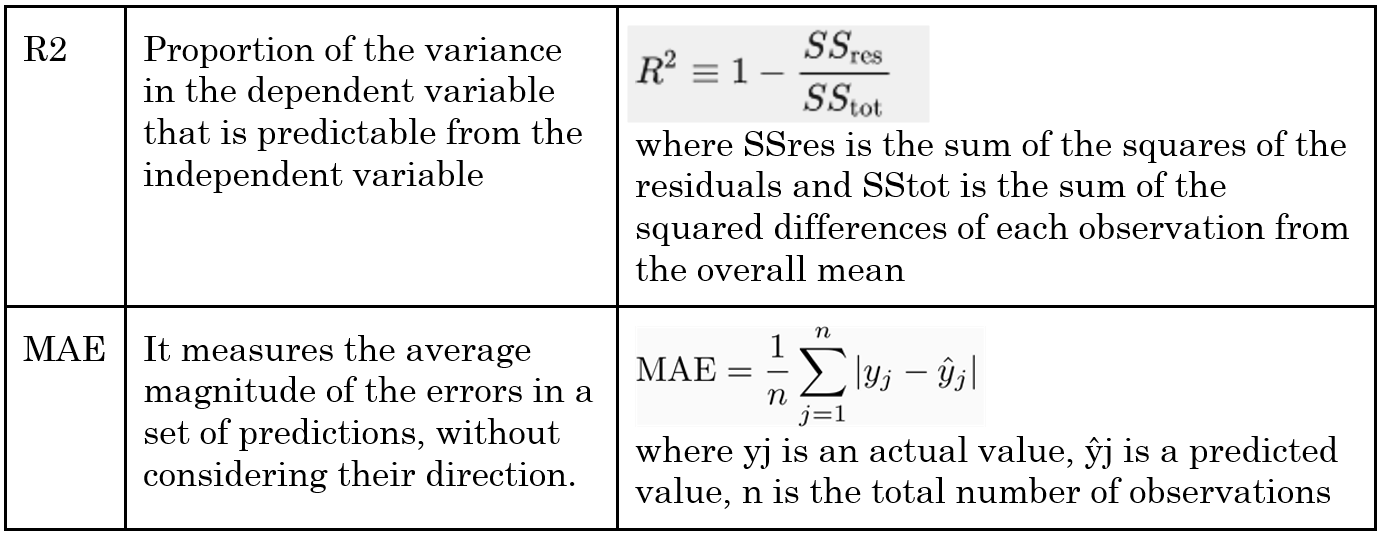
\includegraphics[width=.9\linewidth]{background}
	\caption{Statistical values to evaluate predictions.}
	\label{fig:background}
\end{table}

\section{Data} 
\subsection{Data Generation Experimental Setup}
The laboratory system is a two‐fault configuration that contains fault gouge material submitted to double direct shear (Figure 1)\cite{kaggle}. \par
\begin{figure}[h]
	\centering
	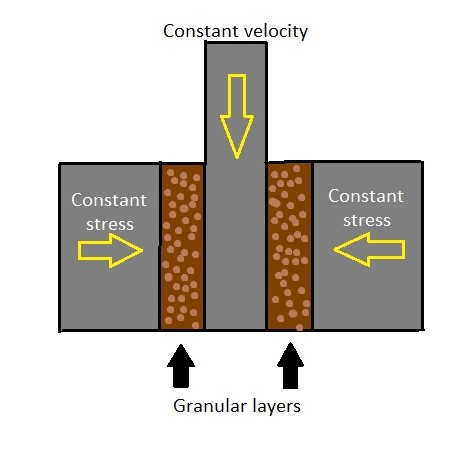
\includegraphics[width=.6\linewidth]{lab}
	\caption{Laboratory Earthquake Design}
	\label{fig:lab}
\end{figure}
Two fault gouge layers are sheared simultaneously while subjected to a constant normal load and a prescribed shear velocity \cite{kaggle}. The laboratory faults fail in repetitive cycles of stick and slip that is meant to mimic the cycle of loading and failure on tectonic faults \cite{kaggle}. While the experiment is considerably simpler than a fault in the Earth it shares many physical characteristics \cite{kaggle}. \par

A driving piston displaces at a very constant velocity during the inter-event time and accelerates briefly when a slip occurs \cite{Bertrand}. An accelerometer records the acoustic emission emanating from the shearing layers \cite{Bertrand}. The steel blocks are extremely stiff therefore the deformation takes place largely in the gouge \cite{Bertrand}. Under a broad range of load and shear velocity conditions, the apparatus stick‐slips quasi‐periodically for hundreds of stress cycles during a single experiment and in general follows predictions from rate and state friction \cite{Bertrand}. The rate of impulsive precursors accelerates as failure approaches suggesting that upcoming laboratory earthquake timing could be predicted \cite{Bertrand}. \par

The experimental data has 16 earthquakes. The shortest time to failure is 1.5 seconds for the first earthquake, 7 seconds for the 7th and the longest is around 16 seconds. \par

\subsection{Data Exploration}
The data used in this work is a 157.275 second recording of seismic signals (Table 2). It was recorded at 4MHz hence 629,145,480 data points accompanied by the time remaining in seconds until the following lab earthquake.\par
The seismic signals are recorded using a piezoceramic sensor which outputs a voltage upon deformation by incoming seismic waves (henceforth we will use the term acoustic signal). The seismic data, which serves as the input to our analysis, is this recorded voltage, in integers. \par

Acoustic signal is voltage upon deformation by incoming seismic waves. \par
Time to failure is the remaining time in seconds until an actual stick-slip failure occurred. \par

\begin{table}
	\begin{center}
		\caption{5 record sample of the data used in this study}
		\label{tab:SampleData}
		\begin{tabular}{c|r} 
			\textbf{Acoustic Signal} & \textbf{Time to Failure}\\
			\hline
			12 & 1.469099998474121 \\ 
			6 & 1.469099998474121 \\ 
			8 & 1.469099998474121 \\ 
			5 & 1.469099998474121 \\ 
			8 & 1.469099998474121 \\ 
		\end{tabular}
	\end{center}
\end{table}
\begin{figure}
	\centering
	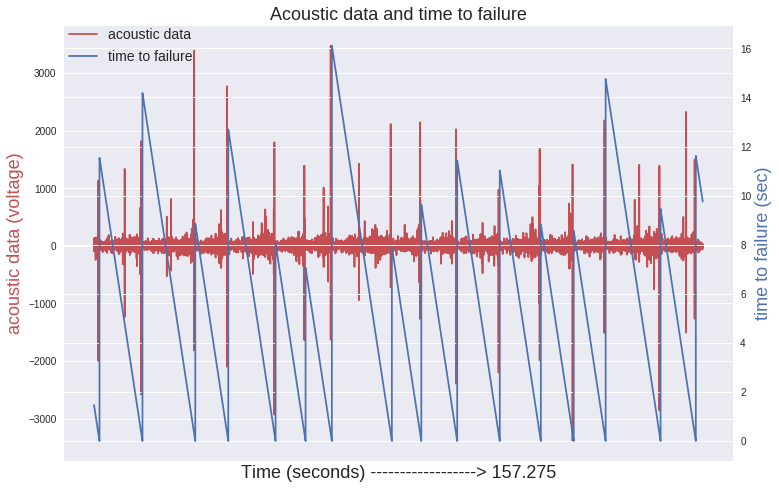
\includegraphics[width=.9\linewidth]{timeSeries}
	\caption{We can see that the acoustic signal shows huge fluctuations regularly just before the failure. It is also worth noting that failures can be predicted visually as cases when huge fluctuations in the signal are followed by smaller signals.}
	\label{fig:timeseries}
\end{figure}
\begin{figure}
	\centering
	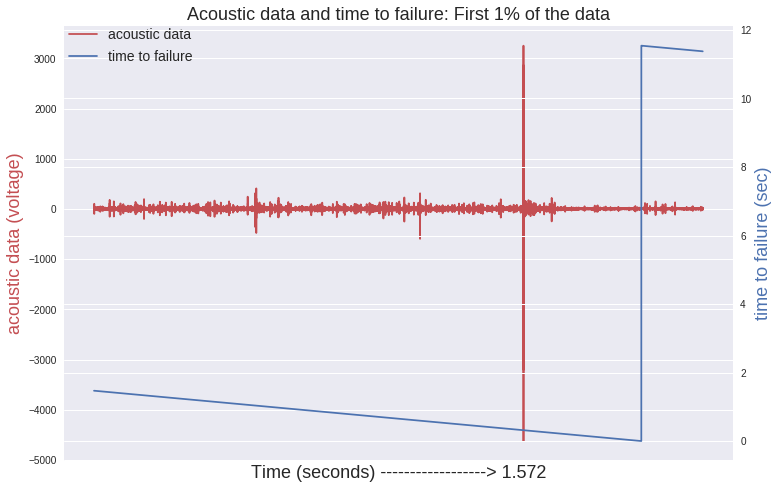
\includegraphics[width=.9\linewidth]{zoomedInTimePLot}
	\caption{On this zoomed-in time plot we can see that the large acoustic signal oscillation at the 1.572 second mark is not at the exact time of the failure but  just before it. There are trains of intense signal oscillations preceding the large one and some smaller ones after it.}
	\label{fig:zoomeInTimePlot}
\end{figure}
\begin{figure}
	\centering
	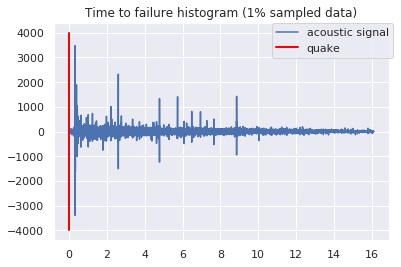
\includegraphics[width=.8\linewidth]{timeToFailureHistogram}
	\caption{In this 1\% sample of the data we can see that the voltage amplitude of acoustic precursors accelerates as failure approaches, suggesting that upcoming laboratory earthquake timing could be predicted. The red line indicates that a quake occurs when the time to failure approaches 0. The minimum time remaining until the quake is -5.5150e+03 sec.}
	\label{fig:timeToFailureHistogram}
\end{figure}
\begin{figure}
	\centering
	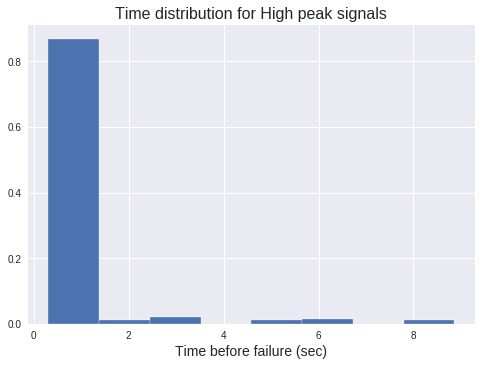
\includegraphics[width=.8\linewidth]{timeDistribution}
	\caption{We found that more than 90\% of high acoustic signal values (absolute value greater than 1000 voltages) are around 0.31 seconds before an earthquake.}
	\label{fig:timeDistribution}
\end{figure}
\begin{figure}
	\centering
	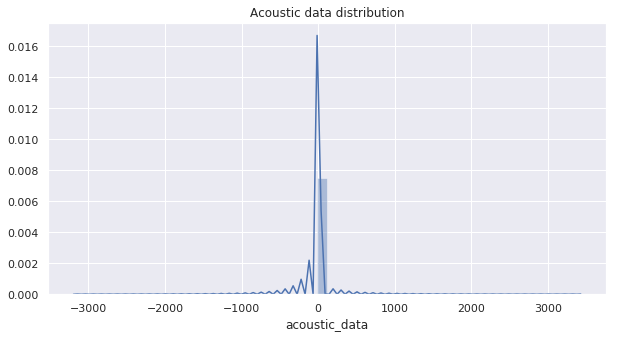
\includegraphics[width=.9\linewidth]{acousticDataDistribution}
	\caption{The distribution of the acoustic signals have a very high peak and we see outliers in both directions.}
	\label{fig:acousticDataDistribution}
\end{figure}
\begin{figure}
	\centering
	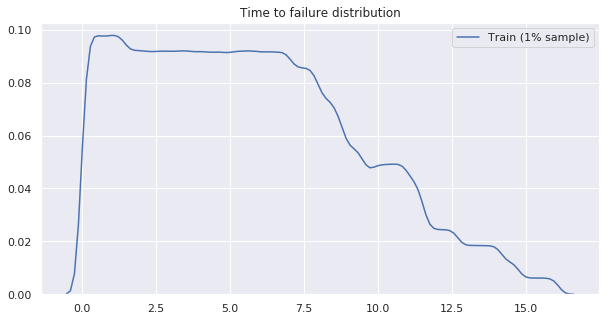
\includegraphics[width=.9\linewidth]{timeToFailureDistribution}
	\caption{The distribution of the time to failure is right skewed.}
	\label{fig:timeToFailureDistribution}
\end{figure}

\clearpage
\newpage
\section{Feature Engineering}
Working with quasi periodic seismic signals LANL achieved a 0.89 coefficient of determination. They divided the data into 1.8 second time windows and used a Random Forest technique. \cite{Bertrand}. The most important features in the LANL model were variance, kurtosis and threshold. \par
We used a similar approach in this study. Our goal is to predict the time remaining before the next failure using only moving time windows of the acoustic data. We divided the data into 0.3 second time windows (1,500,000 observations) which is small enough relative to the lab quake cycle which spans 8 to 16 seconds. As indicated in figure 6 more than 90\% of high acoustic values (absolute value greater than 1000) are around 0.31 seconds before an earthquake. It makes sense to divide our data by 0.3 sec windows to reduce error at the end of the quake cycle. 

\begin{figure}
	\centering
	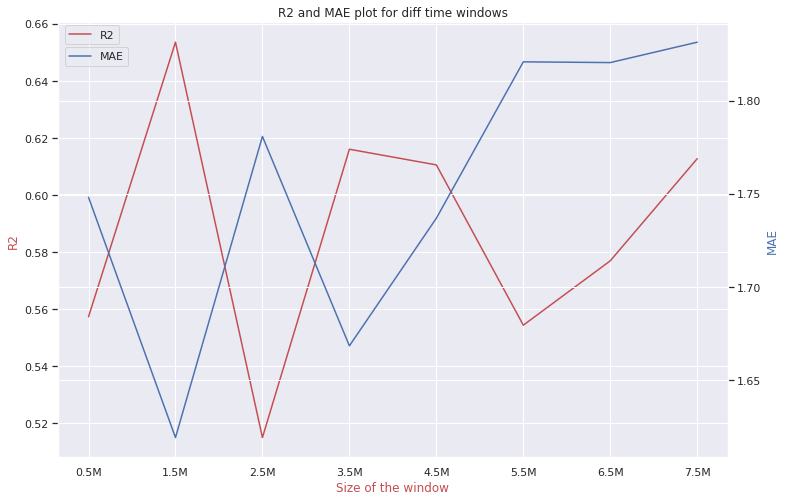
\includegraphics[width=.9\linewidth]{rSquaredandMAE}
	\caption{Checking how sensitive our results are to the size of the time window we find that the highest $r^2$ and smallest mean absolute error we were able to achieve is with 1.5M observations in each time window.}
	\label{fig:rSquaredandMAE}
\end{figure}

Our resulting transformed data set consists of 419 time windows (0.3 seconds each).  From each time window we compute a set of 95 potentially relevant statistical features (e.g., mean, variance, kurtosis, min/max, threshold and so on). Using feature importance technique (a feature is “important” if shuffling its values increases the model error) we found that only the following (in Table 2) are considerably important:
\begin{table}[H]
	\begin{center}
		\caption{List of Engineered Features}
		\label{tab:engineeredFeatrures}
		\begin{tabular}{l} 
Standard Deviation \\
90\% Quantile \\
95\% Quantile \\
99\% Quantile \\
Absolute Standard Deviation \\
Average Rolling Standard Deviation for 100, 1000 and 10000 observations \\
Variance of Rolling Standard Deviation for 100, 1000 and 10000 observations \\
Minimum Rolling Standard Deviation for 100, 1000 and 10000 observations \\
1\% Quantile of rolling standard deviation for 100, 1000, 10000 observations \\
5\% Quantile of rolling standard deviation for 100, 1000, 10000 observations \\
10\% Quantile of rolling standard deviation for 100, 1000, 10000 observations \\
90\% Quantile of rolling standard deviation for 100, 1000, 10000 observations \\
95\% Quantile of rolling standard deviation for 100, 1000, 10000 observations \\
99\% Quantile of rolling standard deviation for 100, 1000, 10000 observations \\
Variance of Rolling Absolute Mean for 100, 1000 and 10000 observations \\
		\end{tabular}
	\end{center}
\end{table}

We apply different machine learning techniques such as the Random Forest Regressor, XGB Regressor,  Decision Tree Regressor, LGBM Regressor and Extra Trees Regressor to the new continuous values that we created analyzing acoustic time series data. \par
To avoid correlation between the new features we applied a principal component analysis technique: orthogonal transformation to convert a set of observations of possibly correlated variables into a set of values of linearly uncorrelated variables. The principle components allows us to reduce the number of features from 35 to only 5 which represents 99.9\% of the full data variation. \par
We use a 50/50 continuous split of the data for use as training and testing data sets respectively. Contiguity of the train and test data sets is important to minimize contamination of the training data with information about the test data. \par
We selected regularization hyper-parameters for each machine learning algorithm using random grid search technique based on a 3-fold cross-validation.
%\clearpage
%\newpage
\section{Results}
We run the ADA Boost and Random Forest Regression techniques on 50\% of the entire data set (training data) before principal component analysis and after. The principal component analysis did not allow for any significant improvement in our results (Figures 9-12). We apply our model to generate predictions on the test data and measure the accuracy of them using $r^2$ and $MAE$ (described in Table 1). \par 

The most accurate results were achieved by the Random Forest algorithm with 1,61 seconds MAE and 0.65 $r^2$. The parameters used are displayed in table 3. %Add Scitkitlearn definitions? Add top background definitions as well? 
The hyper-parameters used with the algorithm  were:

\begin{table}
	\begin{center}
		\caption{Random Forest Parameters}
		\label{tab:hyperparameters}
		\begin{tabular}{l|l} 
			\textbf{Parameter} & \textbf{Setting}\\
			\hline
			Maximum Depth & 10 \\ 
			Maximum Features & log2 \\ 
			Minimum Samples Leaf & 2 \\ 
			Minimum Samples Split & 2 \\ 
			Number of Estimators & 1000 \\
		\end{tabular}
	\end{center}
\end{table}

\par

\begin{figure}
	\centering
	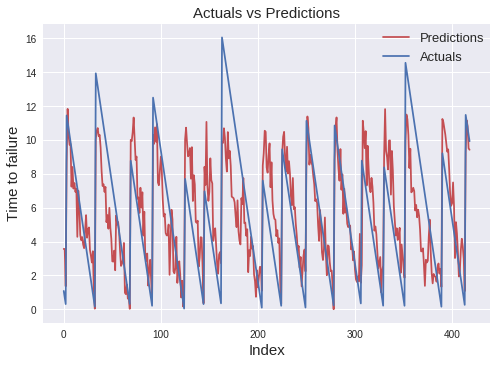
\includegraphics[width=.9\linewidth]{results1}
	\caption{Results achieved with Random Forest Regressor are 1.65 MAE and 0.63 $r^2$. We emphasize that there is no past or future information considered in calculating the predictions (red line). Each prediction uses only the acoustic signal information within one single time window.}
	\label{fig:results1}
\end{figure}

\begin{figure}
	\centering
	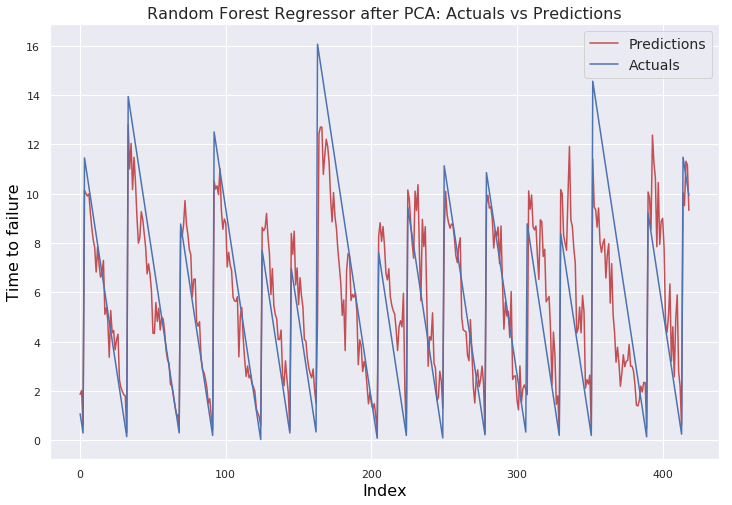
\includegraphics[width=.9\linewidth]{results1PCA}
	\caption{After applying the principle components analysis Random Forest Regressor MAE score is 1.78 and $r^2$ decreased to 0.57.}
	\label{fig:results1PCA}
\end{figure}

\begin{figure}[H]
	\centering
	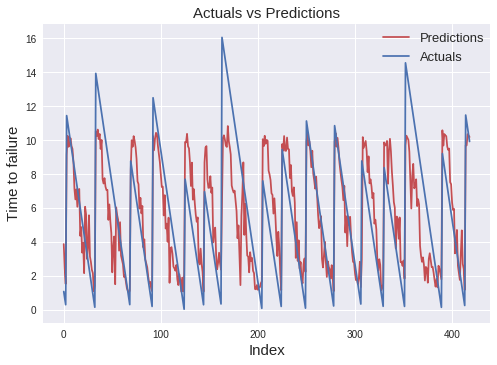
\includegraphics[width=.9\linewidth]{results2}
	\caption{Results achieved with the Ada Boost Regressor algorithm are 1.68 MAE and 0.62 $r^2$ score. The hyper parameters used are learning rate = 0.035421, loss = square, number of estimators = 500 and base estimator= Ridge(alpha=1).}
	\label{fig:results2}
\end{figure}

\begin{figure}[H]
	\centering
	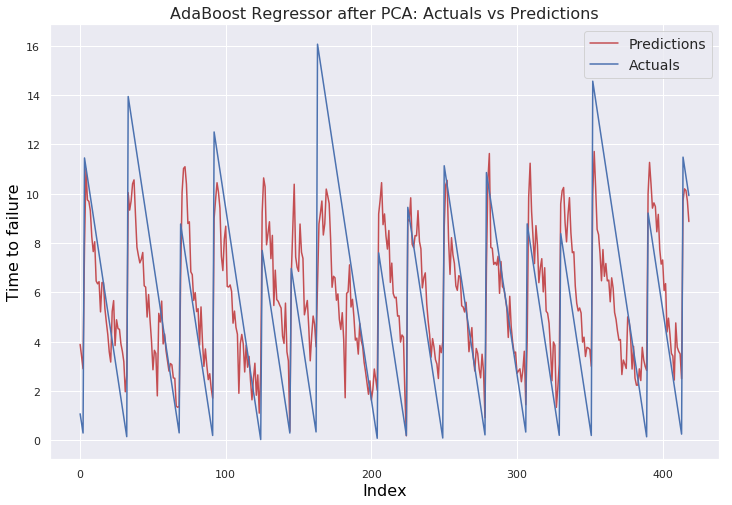
\includegraphics[width=.9\linewidth]{results2PCA}
	\caption{After applying the principle components analysis Ada Boost Regressor results are 1.72 MAE and 0.63 $r^2$ score.}
	\label{fig:results2PCA}
\end{figure}


\clearpage
\newpage
\section{Analysis}
The most accurate results with coefficient of determination 0.63 and mean absolute error 1.65 seconds we achieved using the Random Forest algorithm. The most important features are shown in Figure 14. The top 4 are 90\% and 95\% quartile rolling standard deviations, standard deviation of rolling absolute mean and average rolling standard deviation.
%$SD = \sqrt{\frac{1}{N-1} \sum_{i=1}^N (x_i - \overline{x})^2}$
\begin{figure}[H]
	\centering
%	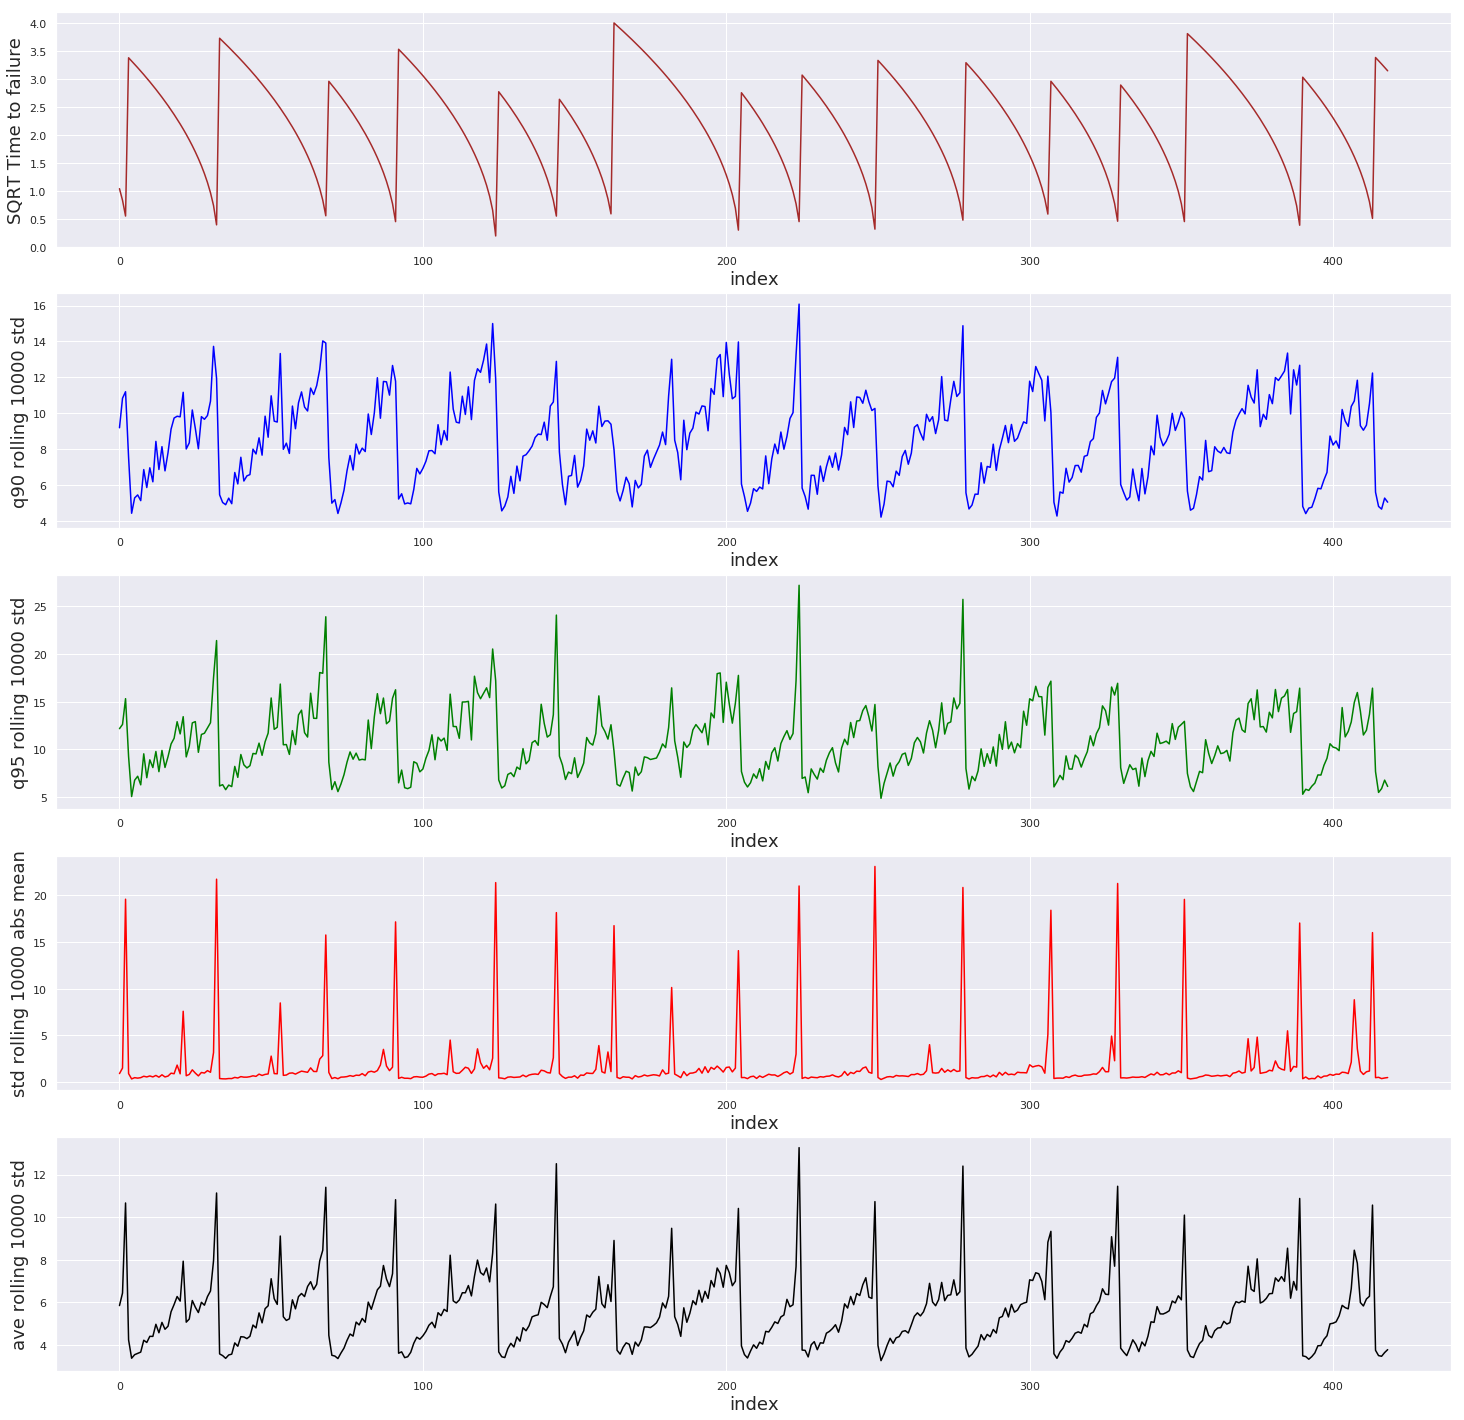
\includegraphics[width=14cm,height=14cm,keepaspectratio]{analysis}
	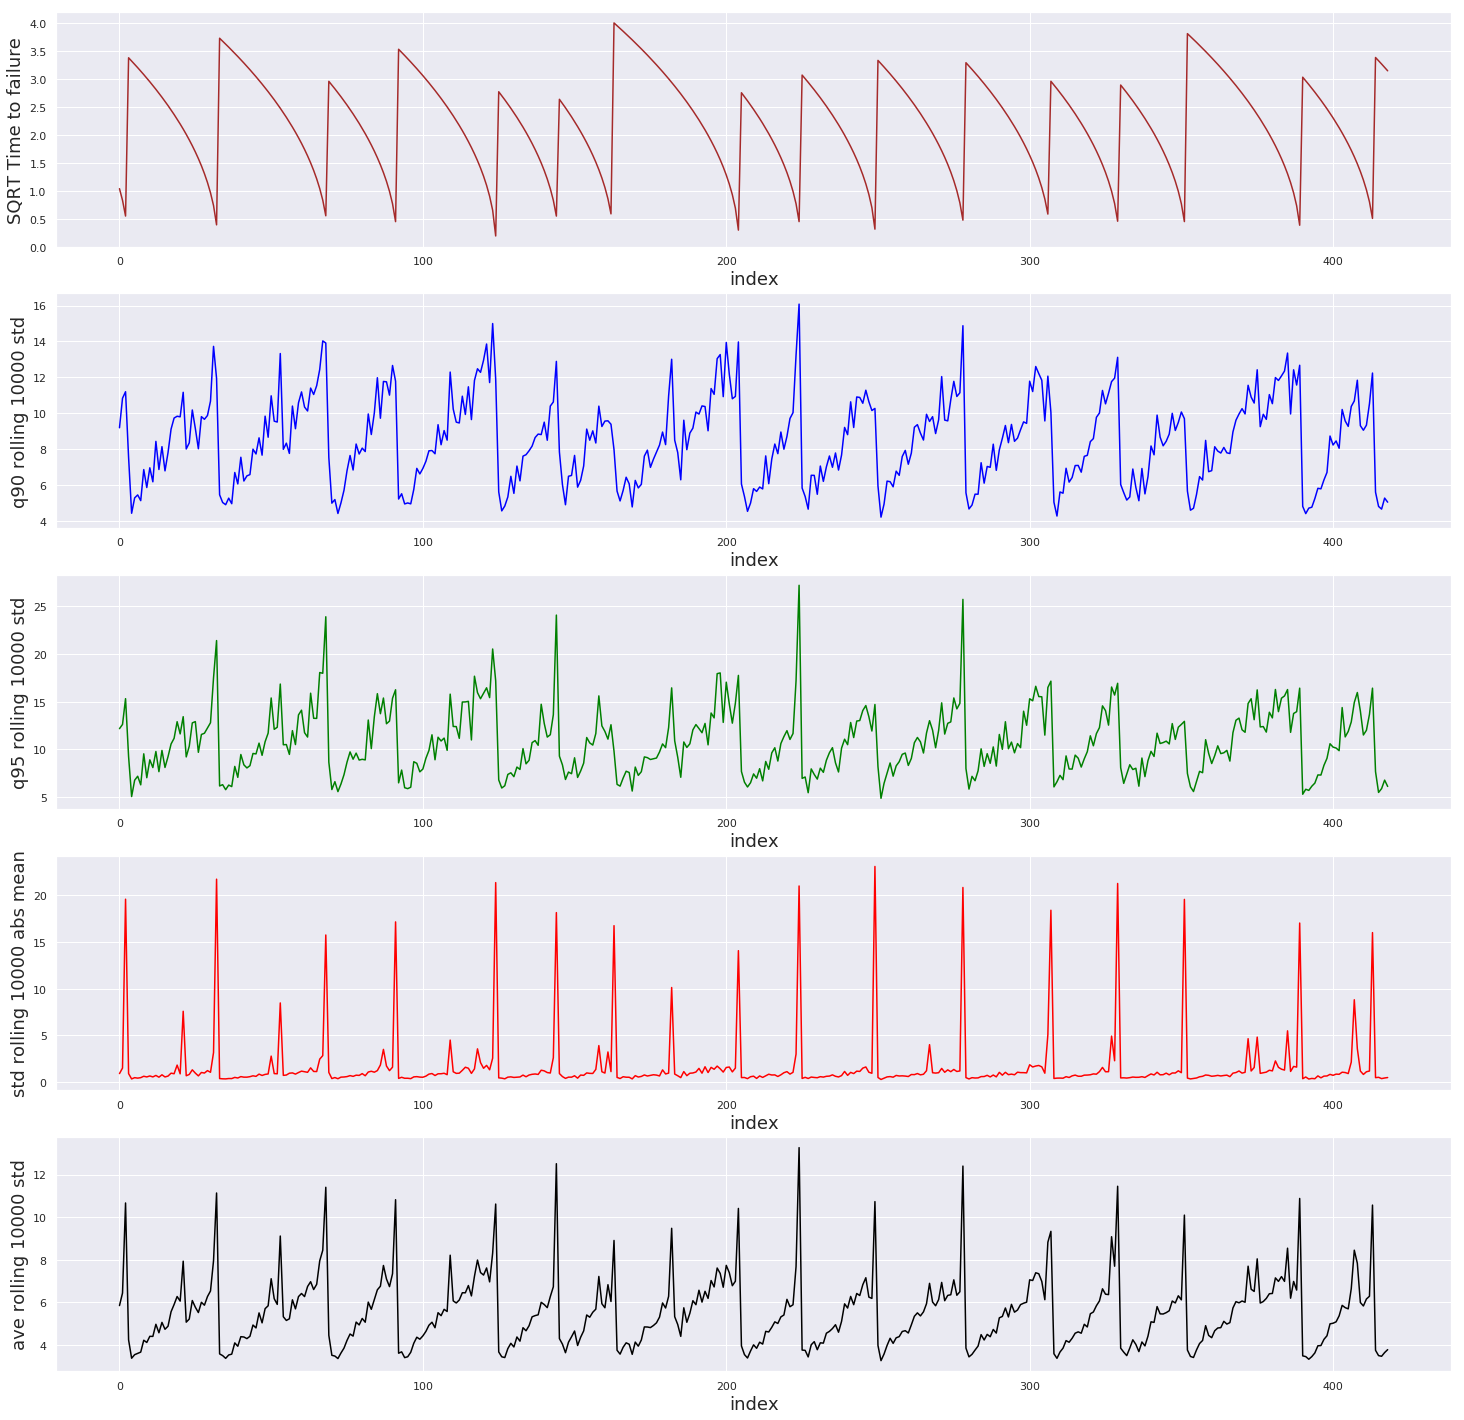
\includegraphics[width=1\linewidth]{analysis}
	\caption{The top 5 data features used to model the predictions.}
	\label{fig:analysis}
\end{figure}

\clearpage
\newpage

\section{Ethics}

Clarence R. Allen, the chairman of the National Earthquake Prediction Evaluation Council claimed that keeping information, from the public and discussing hypotheses on earthquake prediction “behind closed doors” would cause more harm than good, for free speech is the only means to promote research and to increase public responsibility of scientists \cite{Ayhan}. The public’s demand for accurate information would encourage scientists to further their research and hinder them from making unwarranted statements that may cause disturbance in society \cite{Ayhan}. Allen seems to suggest that free scientific communication in its due course would bring order to the scientific environment by eliminating unwarranted scientific hypotheses and predictions, together with the guesses of amateurs and cranks \cite{Ayhan}. \par 

This very paper is evidence of our agreement with Allen's claims (this is indeed a publication). While we hope that the methods presented in this paper can eventually be scaled to real world earthquakes, it is unlikely that these methods will cause public disturbance as they apply only to \emph{laboratory} earthquakes. Also while 8-16 seconds initially seems to be very short notice relative to other natural disaster predictions we must also consider that information can be distributed to masses faster than ever before in our society using current technology.  \par

In this study we follow the principles of the Association for Computing Machinery (ACM) Code of Ethics and Professional Conduct \cite{ACM} to ensure both privacy and security of individuals, and other codes of conduct related to good ethical practices. Ethical principles to make no harm, be honest and trustworthy, respect the work required to produce new ideas were used in our work. We also took professional responsibilities to achieve high quality in both the processes and professional work, maintain high standards of professional competence, accept and provide appropriate professional review, know and respect existing rules pertaining to professional work. \par

\section{Conclusions}

Given aperiodic earthquake failures data set with more akin to the observed behavior of natural earthquakes Machine Learning can provide failure forecasts based on small windows of time up to 16 seconds in advance. The acoustic signal measurement is an indicator of imminent failure. The prior recurrence interval is not needed to make a prediction. The Random Forest machine learning technique provides the most accurate results.

In this study we use only 157 seconds of the data that present 16 failures. Future work should introduce higher volumes of data to determine if accuracy can be improved. Also the combination of the acoustic signal and the recurrence interval should be tested to determine it's affect on accuracy.

\section{Acknowledgment}
The authors thank Dr. Michael L. Blanpied, U.S. Geological Survey, for advice and reviews that greatly improved our work.

%References
\bibliographystyle{splncs}
\bibliography{myBibliography}

\end{document}
